\documentclass{acmtog} 

\usepackage{color}

\usepackage[utf8]{inputenc}
\usepackage{algorithm}
\usepackage{algorithmic}
\usepackage{indentfirst}
\usepackage{subfig}
\renewcommand{\algorithmicrequire}{ \textbf{Input:}}      
\renewcommand{\algorithmicensure}{ \textbf{Output:}}
\begin{document}



\title{Minimizing Online Service Chain Scheduling Cost on Multi-Core Servers} % title

\author{Sihui Xu {\upshape and} Xiangyu Lin
\affil{Shanghai Jiao Tong University}
}
\maketitle


\begin{abstract}
\textbf{ABSTRACT: } Our project is in the field of Software Defined network (SDN). What we mainly focus on is Network Function Virtualization (NFV). NFV is a novel paradigm that enables flexible and scalable implementation of network services on cloud infrastructure. A key factor in the success of NFV is the ability to dynamically allocate physical resources according to the demand. This is particularly important when dealing with the data plane since additional resources are required in order to support the virtual switching of th packets between the Virtual Network Functions (VNFs). The exact amount of these resources depends on the way service chains are deployed and the amount of network traffic being handled. Thus, orchestrating service chains that require high traffic throughput is a very complex task. Prior art on the service chain deployment in a multi-core system can be impractical due to high overhead and exponential complexity. A central challenge for this problem is how to dynamically determine which service chain needs to be deployed onto which server and which VNF needs to be deployed onto which CPU core in an effective manner. 
\\\indent In this project, we propose a two-stage optimization framework to solve this problem. Our major contribution is the solution to the first stage, which aims to minimize the total number of consumed CPU cores. We then prove its NP-hardness. Based on the proof, we propose an near-optimal approximation algorithm (SA) and compare it with another approximation algorithm we designed (Greedy) to demonstrate its superiority. 
\\\indent For the completeness of the whole project, we also state the second stage. This stage aims to  minimize the overall cost on each server subject to the CPU processing capacity constraints. We propose an online algorithm in this stage, which is our minor contribution to this project. 
\end{abstract}


\section{Introduction}
\noindent\textbf{Background and Motivation: } Network Function Virtualization (NFV) can accelerate network innovation by reducing capital expenses and shortening the renewal cycles. It has the ability to dynamically allocate physical resources according to the demand. By implementing NFV on servers, massive network middle-boxes and network operators are able to provide network functions with much more efficient utilization of dedicate hardware resources.
\\\indent A traditional network function can be replaced by a software service chain implemented on commodity servers with multiple CPU cores. A software service chain usually consists of a set of virtual network functions (VNFs). 
\\\indent Regulations and Internet protocols for NFV, such as OpenFlow in software defined networks (SDN), introduce the rules to dynamically process NFV service chains on servers.
\\\indent Here are some deployment strategies to allocate VNF service chains onto servers. 
\\\indent One simple way of placement is the gather placement, which is demonstrated in fig.1. It allocates all the VNFs of one service chain onto one single server. Note that if we use the gather placement, there must be at least one server that can host all VNFs in one NFV service chain in order for the deployment to be feasible. Therefore, there could be situations where gather placement is not feasible. 
\\\indent The second strategy is the distribute placement, which is demonstrated in fig.2. In this strategy, no two VNFs belong to on NFV service chain can be allocated onto the same server.Note that given a service chain, the number of the servers must be larger than or equal to the number of VNFs in the NFV service chain in order for the deployment to be feasible. Therefore, there also could be situations where distribute placement is not feasible.
\begin{figure}[!h]
\centerline{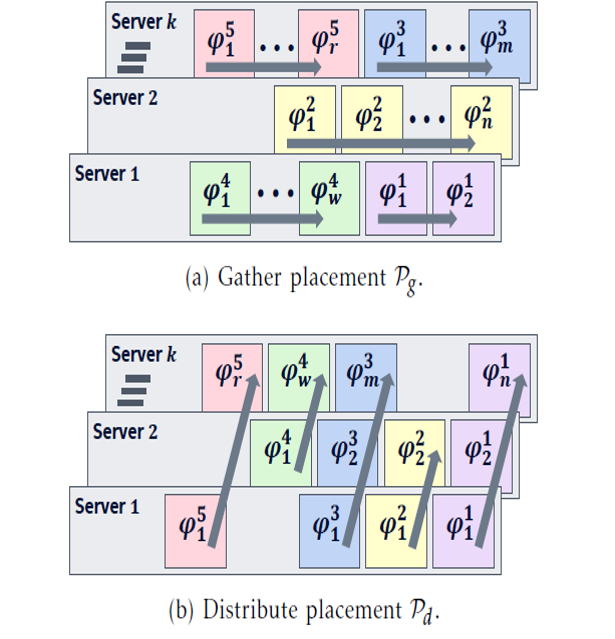
\includegraphics[scale=0.38]{1.png}}
\caption{Gather Placement and Distribute Placement}
\label{fig: gather placement & distribute placement}
\end{figure}
\\\indent In this project, we adopt a more complex and flexible deployment strategy, the arbitrary placement \cite{c1},\cite{c2}. It is a combination of the gather placement and the distribute placement. We decompose a NFV service chain into sub-chains and deploy each sub-chain on a physical server.
\begin{figure}[!h]
\centerline{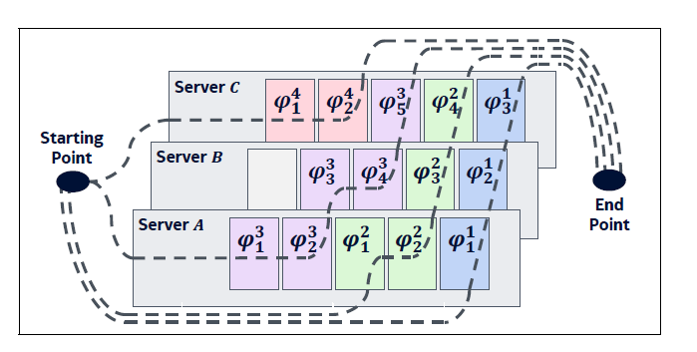
\includegraphics[scale=0.23]{2.png}}
\caption{Arbitrary Placement}
\label{fig: Arbitrary Placement}
\end{figure}
\\\indent However, the algorithm based on partition will result in  an exponential runtime complexity. The exponential runtime complexity will be quite inefficient when confronting with large-scale inputs. In addition, \cite{c1} assumes that different sub-chains are not allowed to be processed on the same server, which is fairly inappropriate since the CPU process is able to migrate between servers in the same cluster freely.
\\\indent In this project, we study a two-stage optimization framework of online NFV service chain scheduling problem on multi-core servers. Given a set of NFV service chains which come in an online manner, we schedule the VNFs and the flow demands in two stages. In the first stage, we divide the coming NFV service chains into sub-chains. Then we process them on different servers to confirm the minimal number of consumed CPU cores. In the second stage, the flow demands come from the solution of the first stage in an online manner. We dynamically steer and schedule the demands for different CPU cores in a server to minimize the overall cost, which involves provision cost and switching cost.


\vspace{1ex}
\\\noindent\textbf{Our Contributions: } We make two contributions in this project. First, we propose a two-stage optimization framework for NFV chain scheduling problem. In the first stage, we aim to minimize the number of occupied CPU cores when the service chains are divided and deployed on different servers. The second stage is dynamic adjustment on CPU cores, aiming at minimizing the overall cost when the demands for VNFs are scheduled on different CPU cores on a certain server.
\\\indent Our second contribution is the solution to the first stage and the second stage. We prove the NP-hardness of the first stage and we design several approximation algorithms and evaluate their performance. Our algorithms run much faster than the algorithm proposed in \cite{c1}. What's more, we have also found an approximation algorithm with near-optimal performance in terms of the minimal cost. Furthermore, inspired by \cite{c3}, we propose an online algorithm based on affine transformation to dynamically steer and schedule the VNF demands on CPU cores.


\section{Related Work}
\indent Due to the page-limitation, we will review the previous art on the NFV service chain scheduling problem briefly.
\\ Ghaznavi et al. \cite{c4} present the concept of operational cost when VNFs are deployed on different servers and provide a method for flexible services. To observe the order in an NFV
service chain, Ma et al. \cite{c5} design a heuristic algorithm to deploy interdependent VNFs, where the relations among these VNFs can be captured by a partially- or totally-ordered set. Breaking free from that one VNF processes all of the flows, Sang et al. \cite{c6} admits that one VNF can process a fraction of one flow while the others can process the rest, whose objective is minimizing the number of running VNF instances. 
\\\indent Recently in the research area for multi-core, NFVnice \cite{c7}  deploys the VNFs of a service chain onto one network function platform with multiple CPU cores, where each VNF is deployed onto one CPU core and different VNFs can share the same CPU core. Besides, Luizelli et al. \cite{c1}\cite{c2} implement to get VNF virtual switching cost and propose an arbitrary placement for NFV service chains, which is a combination of gather placement and distribute placement. On NFV orchestration in an online situation, Wang et al. \cite{c8} study online NFV orchestration and scaling over data centers and provide a learning approach to solve the problem. Shi et al. \cite{c3} put forward a computationally tractable framework for convex optimization with switching costs and ramp constraints and give an implementation on VNF orchestration problems.


\section{Problem Formulation}
In this project, we propose an online two-stage optimization framework to solve the NFV chain scheduling problem.
\subsection{Network Model}
\noindent \textbf{Network:} In this section, we first introduce the network model. We use a directed graph $G=(V,E)$ to present the network, while $V$ represents the nodes in the network and $E$ represents the edges between the nodes in the network.
\\ \textbf{Servers:} We use $S$ to represent the set of multi-core severs in the network, where $S \subseteq V$. Suppose there are totally M servers. For each server $k\in S$ ($1\leq k\leq M$) , we use $S_k$ to denote its number of CPU cores for service chain processing.
\\\textbf{NFV Service Chains: } Then we present our model for the NFV service chains.  We use $\Phi$ to denote the set of the NFV service chains. Suppose there are totally N NFV service chains. Let $\varphi^i$ denote the $i$th NFV service chain, where $1\leq i\leq N$. Then the set of NFV service chains can be formulated as:
$$\Phi = \{\varphi ^1,\varphi ^2,...,\varphi ^N\}$$
\vspace{-2ex}
\\\textbf{VNFs: } An NFV service chain contains several virtual network functions (VNFs). The VNFs are ready to be processed on the servers in the server set $S$. Suppose there are $n_i$ different VNFs for each service chain $\varphi^i$. We use $\varphi^i_j$ to represent the $j$th VNF in NFV service chain $\varphi_i$, where $1\leq j\leq n_i$. Then the set of VNFs in service chain $\varphi^i$ can be defined as:
\vspace{-2ex}
\begin{center}
\begin{equation}
\varphi ^i = \{\varphi ^i_1,\varphi ^i_2,...,\varphi ^i_j,...\varphi ^i_{n_i}\}
\end{equation}
\end{center}
\\\noindent\textbf{Flow Demand: } Then we are going to present the flow demand for each VNF service chain. We denote the number of packets per second for service chain $\varphi_i$ as $p_i$.
\\\noindent\textbf{Computing Resource: } Since different kind of VNFs calls for different amount of computing resource, we use $c^i_j$ to denote the number of consumed CPU cycles to process one packet. If VNF $\varphi^i_j$ is deployed on a CPU core, the consumed CPU cycles per second can be defined as:
\vspace{-1ex}
$$T^i_j=c^i_j\times p_i$$
\vspace{-2ex}
\\\noindent\textbf{Time Slots: } In this problem, the VNF service chains will come in an online manner. We can divide the working time for servers into various time slots. In each time slot, the NFV service chains arrive according to a sequence $t=\{1,2,...,N\}$. At each time t, one NFV service chain $\varphi_t$ comes from a client and the demand should receive response immediately at time t. Therefore, when t reaches N, there have been N NFV service chains in this time slot. And this time slot ends, then a new time slot starts.



\subsection{Problem Definition}
\noindent\textbf{Definition 1. the Two-stage NFV Service Chains Scheduling Problem: } We have a time slot $t={1,2,...,N}$, a set of k servers: $S = \{S_1,S_2,...S_k\}$, and a sequence of service chains: $\Phi = \{\varphi ^1,\varphi ^2...\varphi ^N\}$ which comes in an online manner. Each service chain is a set of VNFs: $\varphi ^i = \{\varphi ^i_1,\varphi ^i_2,\varphi ^1_3,...\varphi ^i_{n_i}\}$. We formulate the problem of the VNF service chains scheduling problem as a two-stage optimization problem. \textbf{First Stage: } In the first stage, we allocate the service chains onto the servers. This stage aims to minimize the number of occupied CPU cores when the VNF service chains are divided into several parts and each part is deployed on different servers. \textbf{Second Stage: } In the second stage, for each server, we dynamically adjust the demands for VNFs on its CPU cores. This stage aims to minimize the total operational cost.








\subsection{Problem Formulation for the First Stage}
\indent Here are our problem formulation for the first stage. In this stage, we allocate NFV service chains to different servers to minimize the total number of occupied CPU cores.
\\\textbf{Sub-chains:} According to Eqn.(1), the NFV service chain comes at time $t$ can be denote as $\varphi^t=\{\varphi^t_1,\varphi^t_2,...,\varphi^t_{n_t},\}$. We divide the NFV service chain into $\Omega$ ($1\leq \Omega \leq N$)VNF sub-chains. We use $\psi^t$ to present the set of sub-chains of $\varphi^t$:
$$\psi^t=\{\psi^t_{s_1\to d_1},\psi^t_{s_2\to d_2},...,\psi^t_{s_w\to d_w},...,\psi^t_{s_{\Omega}\to d_{\Omega}}\}$$
where $\psi^t_{s_{\omega}\to d_{\omega}}$ denotes the $w$th sub-chain
$$\psi^t_{s_{\omega}\to d_{\omega}}=\{\varphi^t_{s_w},\varphi^t_{s_w+1},...,\varphi^t_{d_w-1,}\varphi^t_{d_w}\}$$
where $s_w$ denotes the start of the sub-chain $\psi^t_{s_w\to d_w}$ and $d_w$ denotes the end of the sub-chain $\psi^t_{s_w\to d_w}$. Besides, to maintain the  order of VNF sub-chains, we must follow the constraint:
$$s_{w+1}=d_w+1, \quad \forall\quad 1\leq w\leq \Omega-1$$

\\\indent Then we map each sub-chain to a server. We assume that each VNF can only be routed to one server. Therefore, the set of the sub-chains should be disjoint. Then we have:
$$ \bigcup_{\omega\in[1,\Omega]}\Psi_{s_\omega\rightarrow d_\omega}^t=\boldsymbol{\varphi^t}$$
$$\bigcap_{\omega\in[1,\Omega]}\Psi_{s_\omega\rightarrow d_\omega}^t={\O}$$

\\\noindent\textbf{Allocation Function:} Then we will allocate the sub-chains to the set of servers $S$. We define the allocation function $\mathcal{F}:\psi^t\to S$. If a sub-chain $\psi^t_{s_w \to d_w}$ is allocated to server $k$, we can have $\mathcal{F}(\psi^t_{s_w \to d_w})=k$. When sub-chain $\psi^t_{s_w \to d_w}$ is allocated to server $k$, $\psi^t_{s_{w+1} \to d_{w+1}}$ will not be allocate to the same server $k$, i.e., if $\mathcal{F}(\psi^t_{s_w \to d_w})=k$ and $\mathcal{F}(\psi^t_{s_{w+1} \to d_{w+1}})=k$, we will integrate the two sub-chains into one single sub-chain,i.e.,$\mathcal{F}(\psi^t_{s_w \to d_{w+1}})=k$. To maintain the minimal cost policy, we had better allocate discontinuous sub-chains on one server.


\\\noindent\textbf{Cost of occupied CPU cores: } If we have $\mathcal{F}(\psi^t_{s_w \to d_w})=k$, let $Q$ to represent the cost of occupied CPU cores. According to \cite{c1}, the total cost $Q$ consists of $Q_v$ and $Q_h$. $Q_v$ denotes the required cost to operate VNFs. $Q_h$ denotes the required cost to operate the network traffic switching. According to \cite{c2}, the cost $Q_h$ is defined as:
\vspace{-2ex}
\begin{center}
    \begin{equation}
        \log Q_h(\psi^t_{s_w \to d_w},k)=\alpha_k\times 
        \log(\left| d_w - s_w\right|)+ \beta_k\times 
        \log(p_t)+\gamma_k
    \end{equation}
\end{center}
where $p_t$ is the number of packets per second for service chain $\varphi^t$ and the parameter $(\alpha_k,\beta_k,\gamma_k)$ only depends on the property of server $k$ $(\alpha\in [0,1])$.
\\\indent We use $q^t_j(k)$ to denote the number of consumed CPU cores when VNF $j$ is allocated to server $k$. Then cost $Q_v$ is defined as:
\vspace{-2ex}
\begin{center}
    \begin{equation}
        Q_v(\psi_{s_\omega\to  d_\omega}^t,k) = \sum_{j=s_\omega}^{d_\omega}q_j^t(k)
    \end{equation}
\end{center}
The total number of consumed CPU cores is:
\begin{center}
    \begin{equation}
         Q_(\psi_{s_\omega\to  d_\omega}^t,k) = Q_v(\psi_{s_\omega\to  d_\omega}^t,k)+ Q_h(\psi_{s_\omega\to  d_\omega}^t,k)
    \end{equation}
\end{center}
where $Q_v(\psi_{s_\omega\to  d_\omega}^t,k)$ and $ Q_h(\psi_{s_\omega\to  d_\omega}^t,k)$ is given by Eqn.(3) and Eqn. (4).
\\\textbf{Problem Formulation: }Now we introduce the following problem formulation for the first stage.
\begin{center}
\begin{equation}
\min_{\Omega,(s_\omega,d_\omega),\mathcal{F}}\quad  \sum_{k\in S}   Q(\Psi_{s_\omega\rightarrow d_\omega}^t,k)
\end{equation}
\end{center}



\subsection{Problem Formulation for the Second Stage}
In the second stage, for each VNF demand coming from the solutions of the first stage, we assign them on different CPU cores and dynamically adjust the processing flow rate on each core to confirm the minimal total cost during the time slot $t=\{1,2,\cdots,T\}$ on each server.

\\\indent Here we assume that there are totally $m$ kinds of VNFs and renumber them as $\{\varphi_1,\varphi_2,...,\varphi_r,...,\varphi_m\}$. 
\\\noindent\textbf{Time Set: }We define a time set $T_r^k$ containing the time $t$s in which $\varphi_r$ is allocated to server $k$ in the first stage.

\begin{equation}
  T_r^k(t)=\{t'~|~\mathcal{F}(\Psi_{s_\omega\rightarrow d_\omega}^{t'})=k~and~\varphi_r \in \Psi_{s_\omega\rightarrow d_\omega}^{t'}~and~t'\leq t\}
\end{equation}


\\\noindent\textbf{Flow Rate: }We use $f_r^k(t)$ to denote the total flow rate (which means the total number of packets per second) for VNF $\varphi_r$ on server $k$, which accumulates as time $t$ flows by.Then $f_r^k(t)$ can be formulated as
$f_r^k(t)=\sum_{t \in T_r^k(t)}p_t$


\\\noindent\textbf{Flow Demand: }For a simple CPU core $l$ ($1\leq l\leq S_k$), we use $C_l$ to denote the number of cycles per second when the utility of this CPU core reaches maximum. We assign each demand $f_r^k(t)$ for VNF $\varphi_r$ on different CPU cores and adjust the amount of processing need on each core dynamically as time $t$ goes by. We use $x_{r,l}(t)$ to represent the amount of flow demand of VNF $\varphi_r$ which is processed on core $l$. To satisfy the demand, we have
\begin{equation}
  \sum_{l=1}^k x_{r,l}(t) \geq f_r^k(t) ~\quad \forall r \in [1,m],~\forall t \in [1,T]
\end{equation}
\\\indent Besides, we use $c_{r,l}$ to denote the consumed CPU cycles for processing one packet if VNF $\varphi_r$ is assigned to $l$. In order not to overload the make CPU cores, we have
\begin{equation}\label{CoreConstraint}
  \sum_{r=1}^m c_{r.l}\cdot x_{r,l}(t) \leq C_l,~\quad \forall l \in [1,S_k], ~\forall t \in [1,T]
\end{equation}

\noindent\textbf{Provision Cost: }When the flow demand $x_{r,l}(t)$ are assigned to a CPU core, it will incur a provision cost.
We assume that the server will incur a cost of $\pi_{r,l}$ when a unit of flow demand of $\varphi_r$ are assigned to server $l$. Then the VNF provision cost $W_p^k$ follows\\
\begin{equation}
  W_p^k=\sum_{t=1}^T \sum_{r=1}^m \sum_{l=1}^{S_k} \pi_{r,l}\cdot x_{r,l}(t)
\end{equation}

\noindent\textbf{Switching cost: }We have to endure a cost for the network rerouting when $x_{r,l}(t)$ changes by time $t$. Similar to \cite{shicompetitive}, we use linear switching cost $W_s^k$ to describe the cost for workload balancing and network rerouting. Then we have
\begin{equation}
  W_s^k=\sum_{t=1}^T \sum_{r=1}^m \sum_{l=1}^{S_k} \beta_{r,l}|x_{r,l}(t)-x_{r,l}(t-1)|
\end{equation}
where $\beta_{r,l}$ denotes the switching cost for unit amount of change on $x_{r,l}$. 


\noindent\textbf{Ramp Constraint: }We also introduce the Ramp Constraint in \cite{c3} to limit the amount of network rerouting:
\begin{equation}\label{RampConstraint}
  |x_{r,l}(t)-x_{r,l}(t-1)|\leqslant \Delta x,~\quad \forall~ t,r,l
\end{equation}

\noindent\textbf{Problem Formulation: } 

\begin{center}
    \begin{equation}
         \min \quad W_p^k+W_S^k, \quad \forall ~k \in [1,S_k] s.t. (9)(10)(13)
    \end{equation}
\end{center}









\section{Proposed methods}
\subsection{Complexity Analysis for the first stage}
\noindent\textbf{Theorem 1.} The feasibility of first stage is NP-hard.

\noindent $Proof$: First, we list out all possible sub-chains for service chain $\varphi^t$. We use P to denote the set of all possible sub-chains $P=\{\psi^t_{s_w\to d_w}|\psi^t_{s_w\to d_w}\subseteq\varphi^t\}$. Then we construct the set of subsets for a set cover problem. The set of servers is $S=\{1,2,...,k,...,M\}$. We define a new set $Z$ which describes all possibilities of sub-chains deployment using set multiplication. $Z=P\times S=\{z|\forall\quad \psi^t_{s_w\to d_w}\in P, \forall\quad k\in S \}$, where $z$ is also a set: $z=(\psi^t_{s_w\to d_w},k) = \{\varphi^t_{s_w},\varphi^t_{s_{w+1}},...,\varphi^t_{d_w},k\}$. We define a weight $w_z$ for each element $z\in Z$, then we have $w_z=Q_h+Q_v$. Since the number of consumed CPU cores can not exceed the total number of cores $S_k$, we set $w_z = \infty$ if $Q_h + Q_v > S_k$. Then we use the subsets $z$
in set $Z$ to cover the VNF set $\varphi^t$. In this way, we can reduce the first stage problem to the minimal weight set cover problem. Since the minimal weight set cover problem is NP-hard, the first stage problem is thus NP-hard.









\subsection{Solution to the first stage}
\noindent \textbf{Solution 1 - Greedy Algorithm: }
It is intuitive for us to design the first algorithm in the greedy manner. In every iteration $h$, we choose the sub-chain z with the minimal $f(z)$, which is defined as $f_h(z)=w_z/N_h(z)$, where $N_h(z)$ is the number of uncovered elements in subset $z$ after $h-1$ iterations. If VNF $\varphi^t_j$ is covered by both $z_1$ and $z_2$, we use $z_1'$ to replace $z_1$, where $z_1'=z_1-\{\varphi^t_j\}$.
However, the performance of the greedy algorithm cannot live up to our expectation. Therefore, we design another algorithm, the simulated annealing algorithm to further improve the performance.


\vspace{2ex}
\noindent\textbf{Solution 2 - Simulated Annealing Algorithm:}
We then try simulated-annealing for solving partition problems in our first stage. We use the partition of VNF set as the state to work on, note that the sub-chains have no overlaps and the sub-chains cover the whole chain:
\vspace{-2ex}
$$\psi^t=\{\psi^t_{1\to s_1},\psi^t_{s_1+1\to s_2},...,\psi^t_{s_{w-1}+1\to s_w},...,\psi^t_{s_{n-1}+1\to s_n}\}$$
where the partition is initialized as $s_1 = 1$, $s_i = s_{i-1} + 1 \ \forall i \in (1,n]$

For every iteration we randomly choose to combine or to divide with 0.5 probability respectively. "Combine" means randomly choosing two sub-chains, then merge them to form a new sub-chain, for example if we combine $\psi^t_{s_1\to s_2-1}$ and $\psi^t_{s_2\to s_3-1}$, the new sub-chain will be $\psi^t_{s_1\to s_3-1}$. "Divide" means randomly choosing one sub-chains and divide it into two sub-chains. The dividing index is randomly generated. For example. we divide $\psi^t_{s_1\to s_2-1}$ with index $i$, the new sub-chains are $\psi^t_{s_1\to i}$ and  $\psi^t_{i+1\to s_2-1}$.

After combining or dividing, we have obtain an alternative partition  $\varphi^t_{alt}$. Then we calculate the optimal cost $C'$ of the alternative partition $\varphi^t_{alt}$ and use simulated annealing method to decide whether to update $\varphi^t$ with $\varphi^t_{alt}$ or not. 
\begin{algorithm}[H]
\setcounter{algorithm}{0}
\caption{Simulated Annealing for the first stage}
\begin{algorithmic}[1]
\REQUIRE The number of VNFs $n_t$ in service chain;the required CPU cores $q_j^t(k)$ to operate VNF $\varphi_j^t$;the number of packets per second $p_t$; the number of available CPU cores $S_k$ on the $k$th server; the parameters($\alpha_k,\beta_k,\gamma_k$) for server k.

\ENSURE The partition results of the service chain $\Omega$,($s_w,d_w$); the allocation results $\mathcal{F}$

\STATE Initialize temperature $T$,limit $L$, decay $D$, max iterations per temperature $I$
\STATE Initialize partition of sub chain $\varphi^t =
\{ \{\varphi^t_1\},\{\varphi^t_2\},...\{\varphi^t_{n_t}\}\} $
\STATE Initialize $C$ = optimal cost for $\varphi^t$
\WHILE{$T > L$}
\FOR{Every iteration}
\STATE $\varphi^t_{alt}$ = Randomly combine or divide partitions in $\varphi^t$ once
\STATE $C'$ = the optimal cost for new partition $\varphi'$
\IF{$C' < C$}
\STATE $\varphi^t = \varphi^t_{alt}, C= C'$
\ELSE
\STATE Update $\varphi^t$ and $C$ with $\varphi^t_{alt}$ and $C'$ with probability $exp((C-C')/T)$
\ENDIF
\ENDFOR
\STATE $T = T \cdot D$ for every $I$ iterations
\ENDWHILE
\STATE Obtain $\Omega$, ($s_w,d_w$), $\mathcal{F}$ according to $\varphi^t$
\STATE Return $\Omega$, ($s_w,d_w$), $\mathcal{F}$
\end{algorithmic}
\end{algorithm}
\vspace{-2ex}
Now we are going to analyze the performance of our algorithm-Simulated Annealing algorithm.

\noindent\textbf{Theorem2.} The time-complexity of simulated annealing is $O(n_t^4 \cdot m)$.

\noindent $Proof$: There are  $s_t \in (0,n_t]$ subsets in the current partition for simulated annealing, so the inner loop for every iteration is $M \cdot s_t$, also there are $s_t$ calculation for cost for every iteration. So the inner loop is $M \cdot s_t + s_t^2$. Suppose there are $I$ iterations for every temperature, and there are $a$ iterations for "while" loop, where $a \in [log_{D}\frac{L}{T} \cdot b, \frac{(1+n_t) \cdot n_t \cdot n_t)}{2})$ as $a$ is upper bounded by the total number of possible partitions. The total iteration is $log_{D}(\frac{L}{T}) \cdot b \cdot (M \cdot s_t + s_t^2) + (a - log_{D}(\frac{L}{T}) \cdot b)\cdot (M \cdot s_t + s_t^2) $, the total run time is:
$$
T(n) \leq \frac{(1+n_t) \cdot n_t \cdot n_t)}{2} \cdot M \cdot n_t = O( n_t^4 \cdot M)
$$


\subsection{Solution to the second stage}
In this section, we design an online algorithm based on the framework\cite{c3} to dynamically schedule VNF demands on different CPU cores.

The value of flow rate $f_r^k(t)$ for VNF $\varphi_r$ changes by time $t=\{1,2,\cdots,T\}$ according to the allocation results in the first stage. We must make the decisions $x_{r,l}(t)$ at each time $t$ to observe the demands from clients while minimizing the total provision cost and switching cost. Besides, the introduction of switching cost and the ramp constraint makes our decisions more difficult. 

\\First, we formulate the flow rate $f_r^k(t)$ as a column vector $\bm{f}(t)$ with $m$ components, where $\bm{f}(t) =[~f_1^k(t),f_2^k(t),\cdots,f_m^k(t)~]^T.$
Note that $\bm{f}(t)$ is not a completely arbitrary variable since $\bm{f}(t)$ is generated from the first stage. Although we are able to make reasonable predictions for $\bm{f}(t)$, we don't know it until time $t$. 
\\\indent Our decisions $x_{r,l}(t)$ can also be formulated as a column vector $\bm{X}(t)$ with $m\cdot S_k$ components.
\begin{equation}\label{XVector1}
  \bm{X}(t)=[~\bm{x}_{1,l}(t), ~\bm{x}_{2,l}(t),\cdots ,\bm{x}_{r,l}(t),\cdots,\bm{x}_{m,l}(t)~]^T,
\end{equation}
w $\bm{x}_{r,l}(t)$ follows
\begin{equation}\label{XVector2}
  \bm{x}_{r,l}(t)=[~x_{r,1}(t),~x_{r,2}(t),\cdots,~x_{r,l}(t),\cdots,x_{r,S_k}(t)~]^T.
\end{equation}
\boldmath$x$\unboldmath${}^T$ is the transpose of vector \boldmath $x$ \unboldmath and $\bm{x}_n$ is the $n$th components of vector $\bm{x}$.

At each time $t$, the environment updates the VNF flow demand vector $\bm{f}(t)$, we must update our decision vector $\bm{X}(t)$ and suffer from switching penalties and ramp constraint to confirm the global optimal cost during time $t=\{1,2,\cdots,T\}$.
\\\indent The variables $\pi_{r,l}$ and $\beta_{r,l}$ can also be formulated as vectors $\bm{\pi}$ and $\bm{\beta}$ (both of them possess $m\cdot S_k$ components) according to the regulations mentioned in Eqn.(13) and Eqn.(14). 
\\\indent The capacity $C_l$ of CPU core $l$ can also be formulated as a vector $\bm{C}=[C_1,C_2,\cdots,C_{S_k}]^T$.

\\\indent Here is the standardized form of the second stage:

{\noindent \bf Standardized problem: }\\
\begin{subequations}
\begin{align}
&\min \quad W^k=\sum_{t=1}^{T} \bm{\pi}^T \cdot \bm{X}(t)+\bm{\beta} \cdot|\bm{X}(t)-\bm{X}(t-1)| \\
& s.t. \quad \bm{A^r}\cdot\bm{X}(t)+\bm{A^{r'}}\cdot\bm{f}(t) \leqslant 0,\quad\forall ~r\in[1,m],~\forall~t,\\
& \indent\indent~~\bm{B^l}\cdot \bm{X}(t)+ \bm{B^{l'}}\cdot \bm{C} \leqslant 0,~~~\quad \forall~l\in [1,S_k],~\forall~t,\\
& \indent\indent~~|\bm{X}_n(t)-\bm{X}_n(t-1)| \leqslant \Delta x\quad \forall ~n\in [1,m\cdot S_k].
\end{align}
\end{subequations}


In the standardized problem, $\bm{A^r}$, $\bm{A^{r'}}$, $\bm{B^l}$ and $\bm{B^{l'}}$ are coefficient vectors we can easily calculate by comparing standardize problem with Program (12).

According to \textbf{affine policy} mentioned in \cite{c9}, the vector $\bm{X}(t)$ can be expressed by the linear form of input flow demand $\bm{f}(t)$:
\begin{equation}
  \bm{X}(t)=\bm{b}(t)+\bm{k}(t)\cdot \bm{f}(t)
\end{equation}
where $\bm{b}(t)\in \bm{R}^{(mS_k)}$ and $\bm{k}(t)\in \bm{R}^{(m)\times(mS_k)}$.
Therefore, we can determine $\bm{X}(t)$ from $\bm{f}(t)$ by finding suitable $\bm{b}(t)$ and $\bm{k}(t)$ at each time $t$. We can only optimize the objective value as much as possible, since we do not know the coming $\bm{f}(t)$ in advance.

Therefore, we consider to minimizing the competitive ratio $CR$:
\vspace{-2ex}
$$CR~=~\max_{\bm{f}(t)\in\bm{F}}\frac{W^k(\bm{b}(t), \bm{k}(t) , \bm{f}(t))}{W^k_{off}(\bm{X}(t),\bm{f}(t))}$$
where $W^k_{off}(\bm{X}(t),\bm{f}(t))$ denote the optimal value if we know $\bm{f}(t)$ beforehand. To get an excellent competitive ratio of our online algorithm, we use $CR$ as the objective function instead of $W^k$. Combining the constraints in Standardized problem, we can formulate Affine problem as follows:\\

{\noindent\bf Affine problem: }\\
\begin{subequations}
\begin{align}
&\min_{\bm{b}(t),\bm{k}(t)}~~ CR=\max_{\bm{f}(t)\in\bm{F}}~\frac{W^k(\bm{b}(t), \bm{k}(t) , \bm{f}(t))}{W^k_{off}(\bm{X}(t),\bm{f}(t))}\quad\quad\quad~~ \\
& s.t.\quad\bm{A^r}\cdot\bm{b}(t)+(\bm{A^r}\bm{k}(t)+\bm{A^{r'}})\cdot\bm{f}(t)\leq 0,\forall~r\in[1,m],~\forall~t,\\
& \indent\indent~\bm{B^l}\cdot\bm{b}(t)+\bm{B^l}\bm{k}(t)\cdot\bm{f}(t)+ \bm{B^{l'}}\cdot \bm{C} \leq 0,\forall~l\in [1,S_k],~\forall~t,\\
& \indent\indent|\bm{b}_n(t)-\bm{b}_n(t-1)+(\bm{k}\bm{f})_n(t)+(\bm{k}\bm{f})_n(t-1)| \leq \Delta x,\\
&  ~\quad\quad\quad\quad\quad\quad\quad\quad\quad\quad\quad\quad\quad\quad\quad\qua\quad\quad\forall ~n\in [1,m\cdot S_k],~\forall~t.
\end{align}
\end{subequations}

It is hard to solve the affine problem because the objective function involves a ratio of convex functions. We can use Lemma 1 in \cite{c3} to  transform it to an equivalent convex optimization problem.


First, we define $\mu(t)$ as the upper bound of switching cost $W_s^k$, where
\begin{equation*}
  \mu(t)=\sup_{\bm{f}(t)\in \bm{F}}\bm{\beta}^T|\bm{b}(t)+\bm{k}(t)\bm{f}(t)-\bm{b}(t-1)-\bm{k}(t-1)\bm{f}(t)|
\end{equation*}
. Then we relax the objective function in Affine problem by replacing the switching cost $W_s^k$ in the numerator by $\mu(t)$, then we obtain the relaxed objective function as follows
\begin{equation}
  \min_{\bm{b}(t),\bm{k}(t),\mu(t)}~~ CR'=\max_{\bm{f}(t)\in\bm{F}}~\frac{W^k(\bm{b}(t), \bm{k}(t) , \bm{f}(t)),\mu(t)}{W^k_{off}(\bm{X}(t),\bm{f}(t))}
\end{equation}
Note that the optimal solution remains the same because $W_s^k$ is a convex function of $\bm{f}(t)$. It will not influence the optimal value when the objective function reaches minimal. Then we use Lemma 1 in \cite{c3} to transform it to a convex optimization problem:

{\noindent\bf Convex problem: }\\
\begin{subequations}
\begin{align}
&\min_{\bm{b}(t),\bm{k}(t),\mu(t)}~~\max_{\bm{f'}(t)\in\bm{F},u>0}~  \left\{ W_p^k(\bm{f'}(t))+\sum_{t=1}^{T}\mu(t)u \right\} \quad~~ \\
& s.t. \indent\bm{A^r}\cdot\bm{b}(t)+(\bm{A^r}\bm{k}(t)+\bm{A^{r'}})\cdot\bm{f}(t) \leq 0,\\
& \indent\indent~\bm{B^l}\cdot\bm{b}(t)+\bm{B^l}\bm{k}(t)\cdot\bm{f}(t)+ \bm{B^{l'}}\cdot \bm{C} \leq 0,\forall~l\in [1,S_k],~\forall~t,\\
& \indent\indent|\bm{b}_n(t)-\bm{b}_n(t-1)+(\bm{k}\bm{f})_n(t)+(\bm{k}\bm{f})_n(t-1)| \leq \Delta x,\\
&  ~\quad\quad\quad\quad\quad\quad\quad\quad\quad\quad\quad\quad\quad\quad\quad\quad\quad\quad\forall ~n\in [1,m\cdot S_k],~\forall~t,\\
&  \indent\indent u\cdot W_{off}(\frac{\bm{f'}(t)}{u})\leq 1.
\end{align}
\end{subequations}

\\\indent We can solve the convex problem through Interior Point Method (IPM) in polynomial time. After we get the optimal solution $\bm{b}(t)$ and $\bm{k}(t)$, we use the affine policy to determine $\bm{X}(t)$ according to $\bm{f}(t)$. The algorithm is shown as follows.


\begin{algorithm}[h!]
\setcounter{algorithm}{1}
\caption{An Online Algorithm for the second stage}
\begin{algorithmic}[1]
\REQUIRE The flow demand for each VNF $f(t)$ at time $t$; the set $F$ containing all possible $f(t)$; the consumed CPU cycles for processing one packet $c_{r,l}$; the provision cost $\pi_{r,l}$; the switching cost $\beta_{r,l}$; the maximal CPU cycles $C_l$ for server $l$.
\ENSURE The solution $\{ x_{r,l}(t) \}$
\STATE Initialize the vectors $C(t)$, $\pi(t)$ and $\beta(t)$;
\STATE Solve the convex problem and acquire the optimal $b^*(t)$ and $k^*(t)$;
\FOR{$t=1$ $to$ $T$}
\STATE An $f(t)$ comes from $F$;
\STATE Let $X(t)=b^*(t)+k^*(t)f(t)$;
\STATE Get $x_{r,l}(t)$ according to (13) and (14);
\STATE Return $x_{r,l}(t)$;
\ENDFOR
\end{algorithmic}
\end{algorithm}


\section{Experiments}
\subsection{Experimental evaluation for the first stage}

\begin{figure}[!h]
    \begin{minipage}[t]{0.5\linewidth}
    \centering
    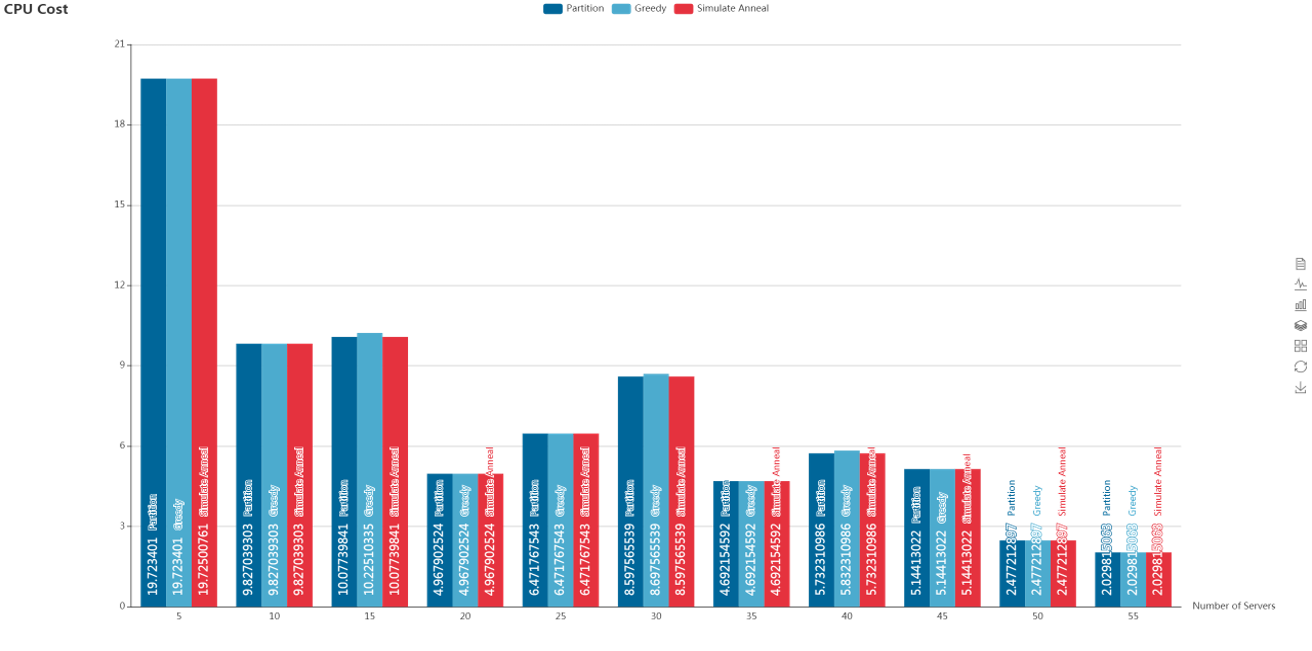
\includegraphics[height=2.4cm,width=3.8cm]{3.png}
    \caption*{(a) CPU cost with different number of servers}
    \label{fig:CPU cost with different number of servers}
    \end{minipage}
    \begin{minipage}[t]{0.5\linewidth}
    \centering
    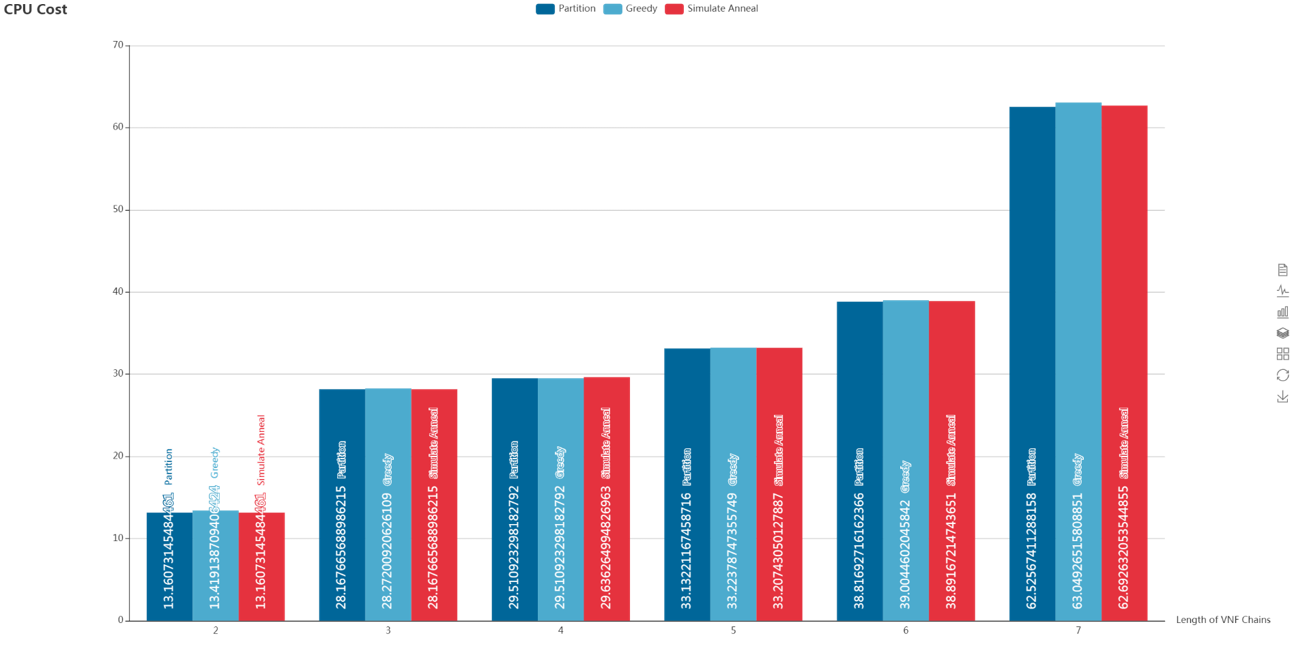
\includegraphics[height=2.4cm,width=3.8cm]{4.png}
    \caption*{(b) CPU cost with different length \\of NFV service chains}
    \label{fig:CPU cost with different length of NFV service chains}
    \end{minipage}
\end{figure}

\begin{figure}[!h]
    \begin{minipage}[t]{0.5\linewidth}
    \centering
    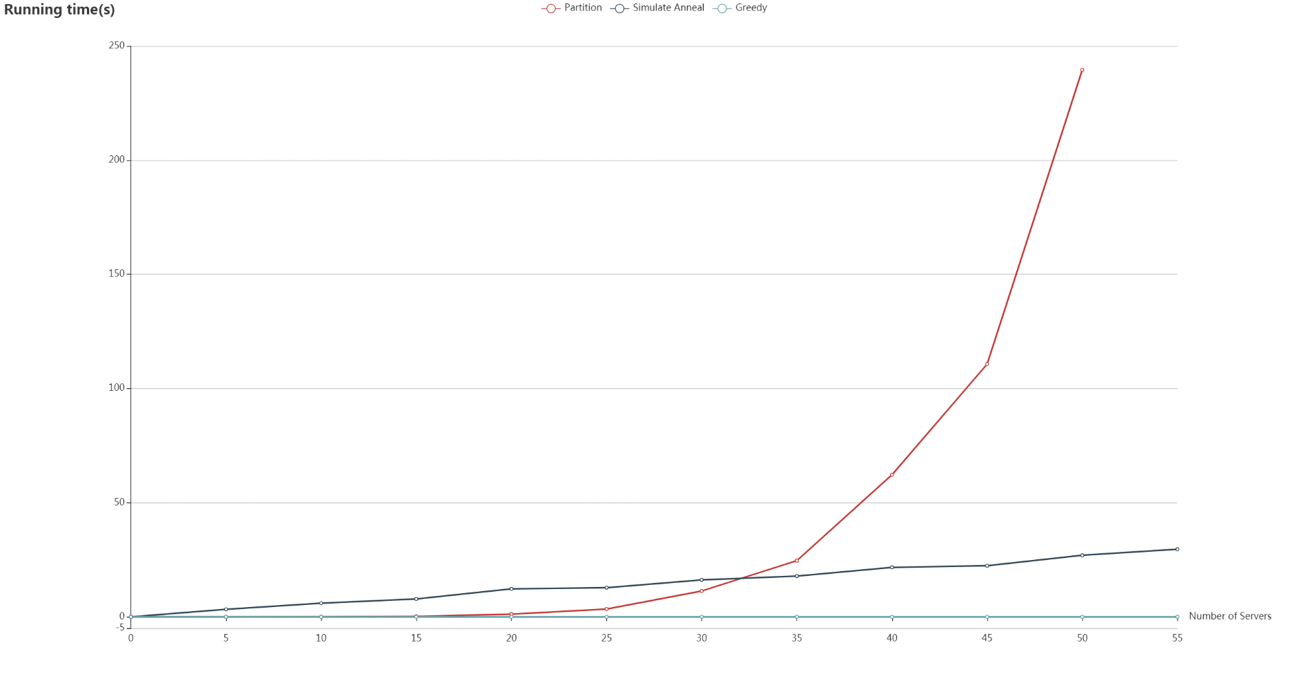
\includegraphics[height=2.4cm,width=3.8cm]{5.png}
    \caption*{(c) Running time with different number of servers}
    \label{fig:Running time with different number of servers}
    \end{minipage}
    \begin{minipage}[t]{0.5\linewidth}
    \centering
    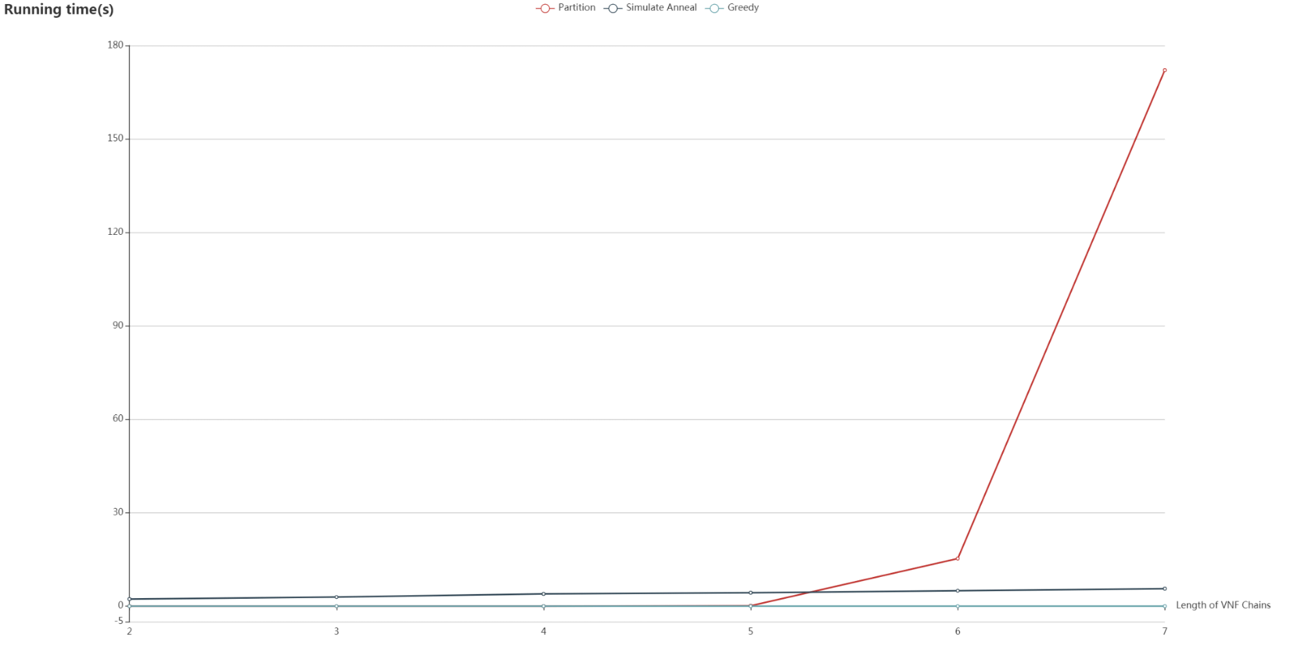
\includegraphics[height=2.4cm,width=3.8cm]{6.png}
    \caption*{(d) Running time with different length of NFV service chains}
    \label{fig:Running time with different length of NFV service chains}
    \end{minipage}
\end{figure}

\begin{figure}[!h]
\centerline{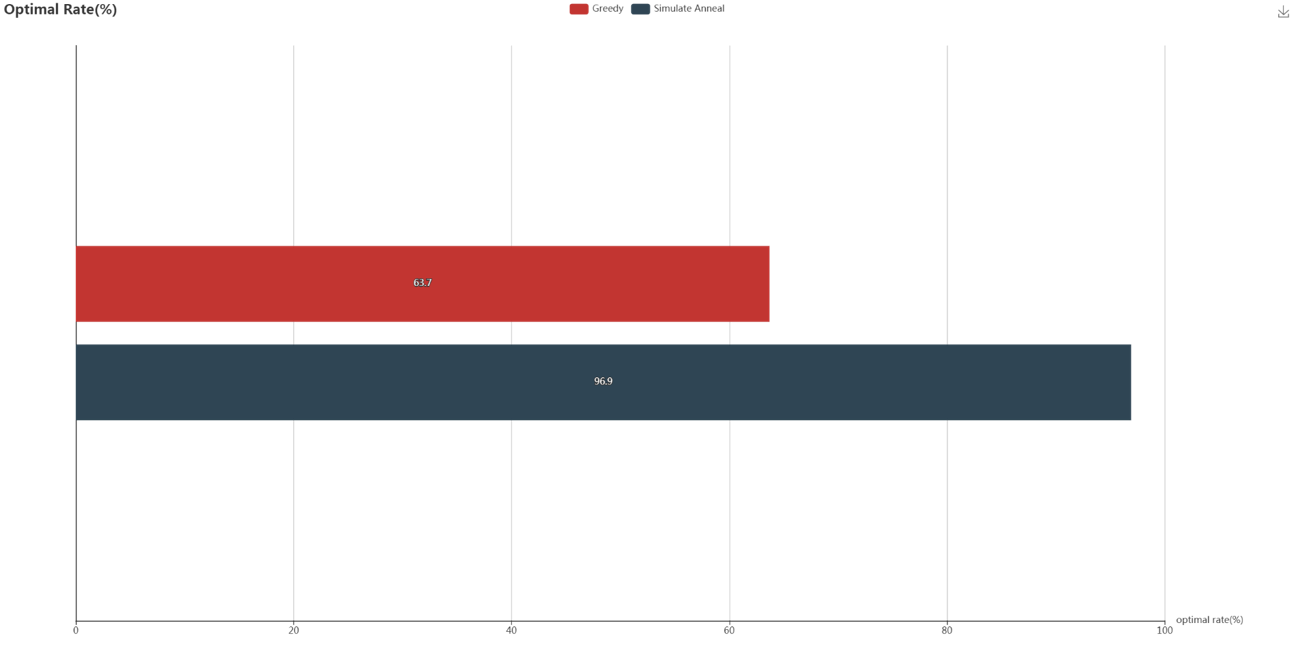
\includegraphics[scale=0.28]{7.png}}
\caption{Optimal rate of the two approximation algorithms}
\label{fig: Optimal rate of the two approximation algorithms}
\end{figure}


In first stage, we did two experiments: changing the number of servers with fixed NFV service chain length 3 and changing length of NFV service chain with fixed server number 10. We record the CPU cost and running time of three algorithms in both experiments.

We then compare the CPU cost and running time of partition, greedy and SA. Partition gives us optimal result all the time, but the running time will increase rapidly as number of servers or number of VNFs grows. Greedy runs the fastest but it suffers from the low optimal rate. SA has a very high chance of getting optimal cost (96.9$\%$), and also has excellent running time when the number of servers or number of VNFs grows.


In addition, we did experiment to compare the chance of getting optimal result of greedy and SA with fixed number of server(17) and fixed length of NFV service chain(3) running for 500 times. Greedy has a 63.7$\%$ optimal rate while SA is near-optimal with 96.9 $\%$ optimal rate.

These results shows that greedy and SA are good approximations for the partition algorithm. Especially SA, which has both outstanding running time and near-optimal performance.

\subsection{Experimental evaluation for the second stage}

\begin{figure}[!h]
    \begin{minipage}[t]{0.5\linewidth}
    \centering
    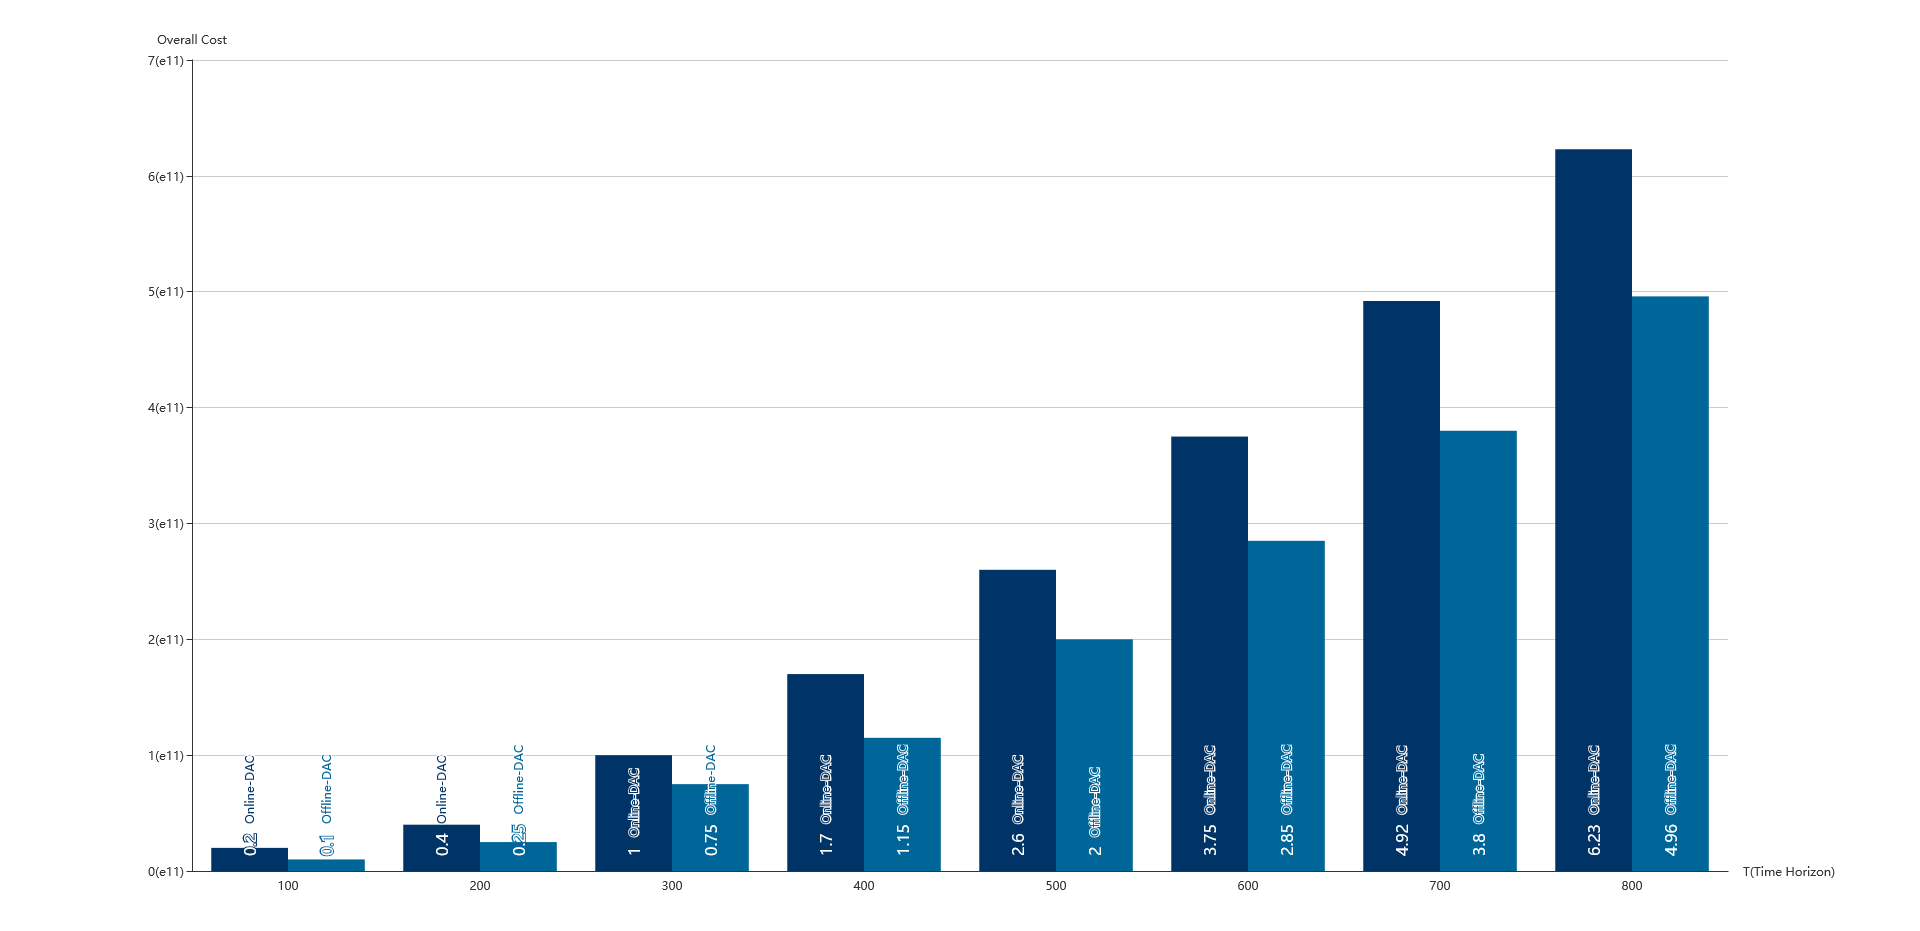
\includegraphics[height=2.4cm,width=3.8cm]{9.png}
    \caption*{(a) Overall cost with different time horizons}
    \label{fig:Overall cost with different time horizons}
    \end{minipage}
    \begin{minipage}[t]{0.5\linewidth}
    \centering
    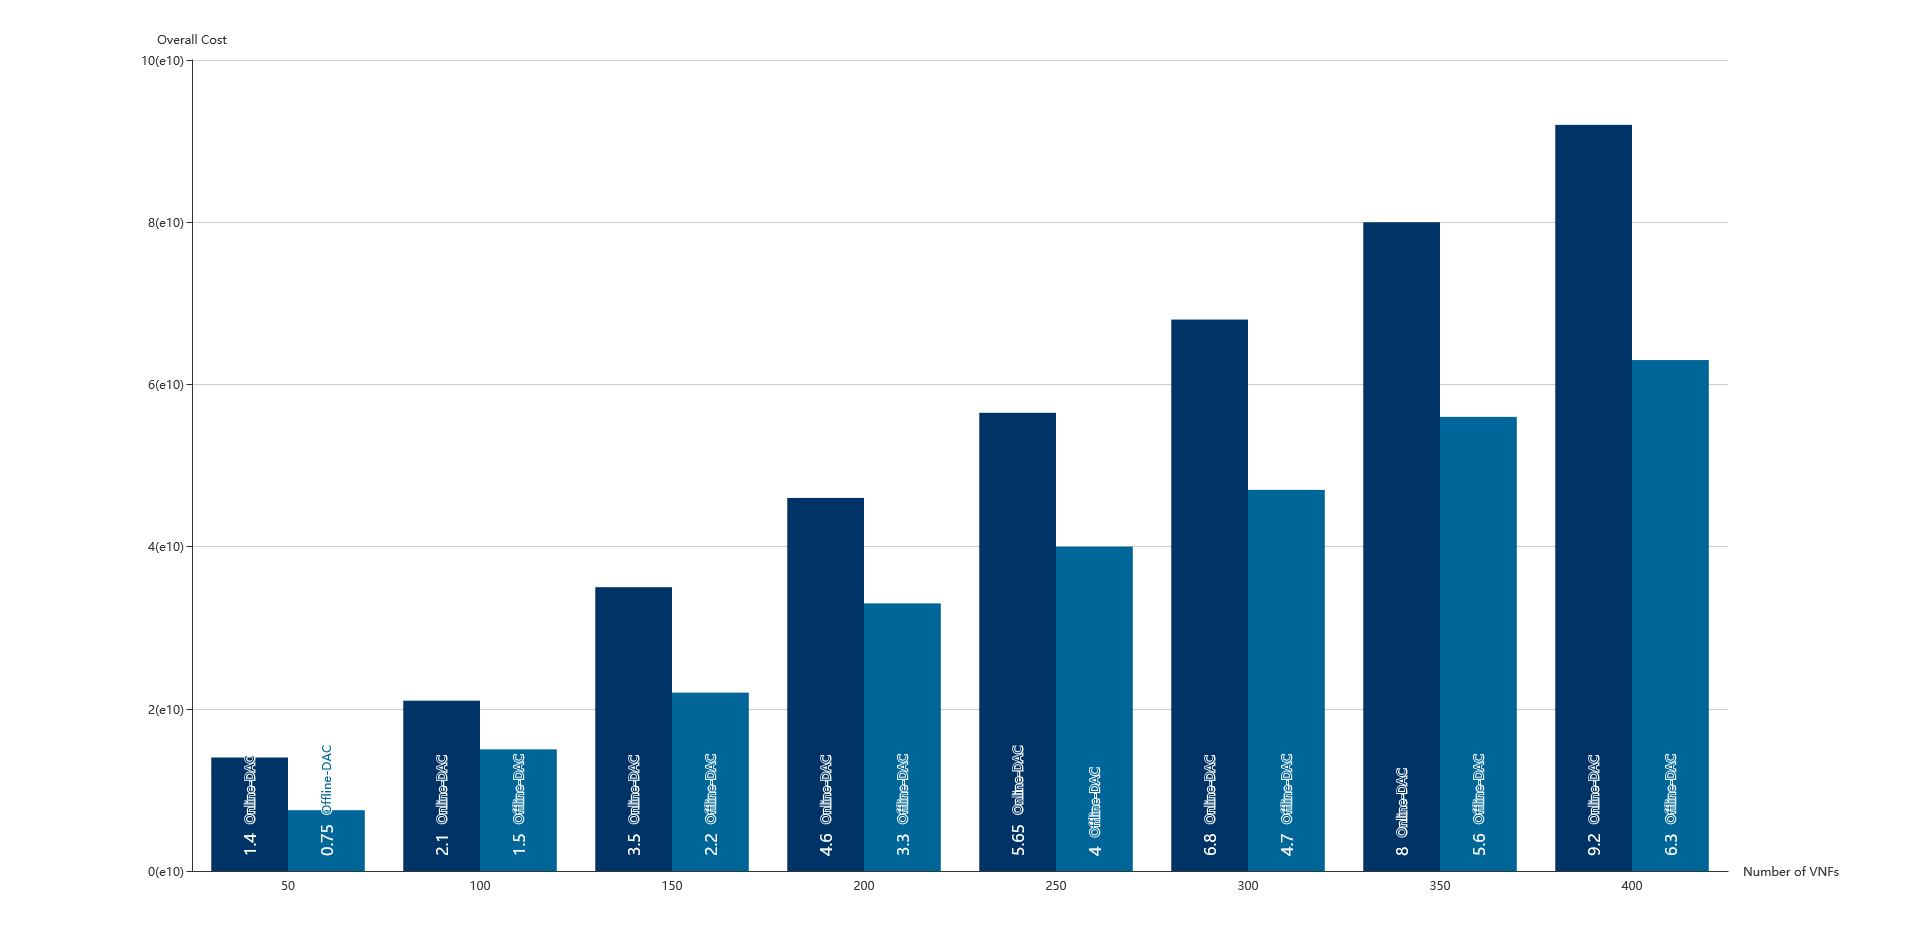
\includegraphics[height=2.4cm,width=3.8cm]{10.png}
    \caption*{(b) Overall cost with different number of VNFs}
    \label{fig:Overall cost with different number of VNFs}
    \end{minipage} 
\end{figure}

\begin{figure}[!h]
    \begin{minipage}[t]{0.5\linewidth}
    \centering
    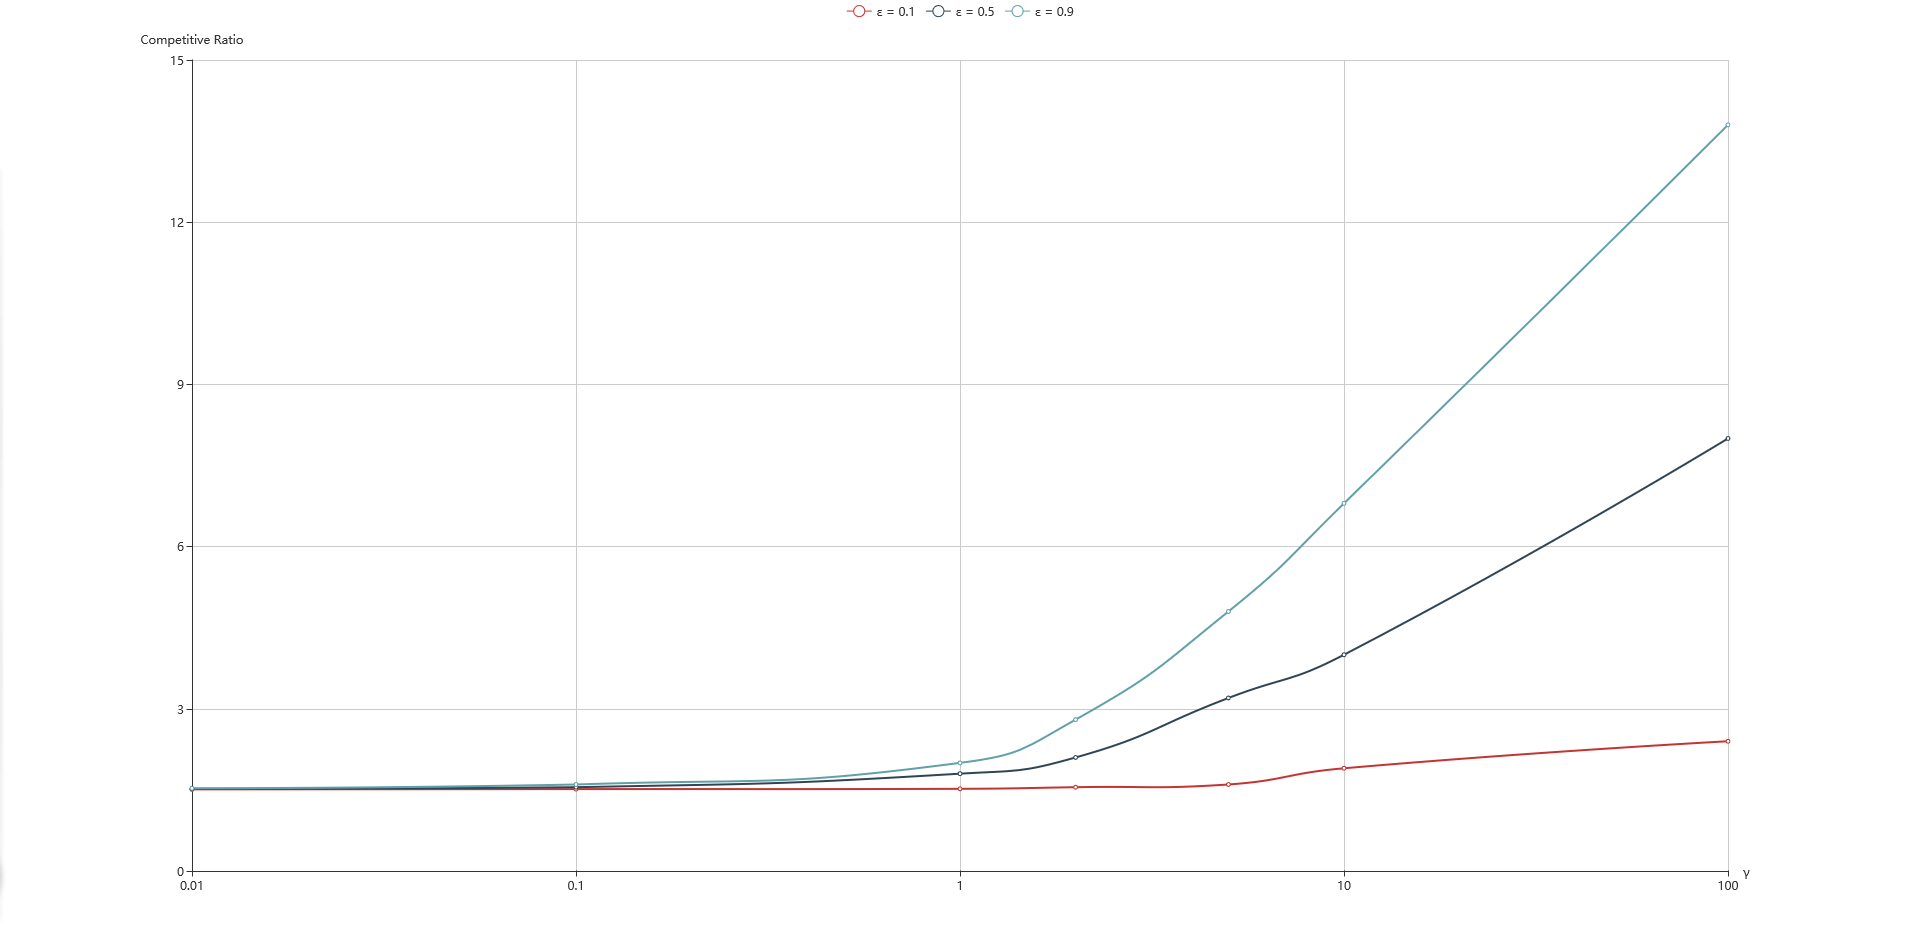
\includegraphics[height=2.4cm,width=3.8cm]{11.png}
    \caption*{(c) Competitive ratio with the ratio between switching cost and provision cost}
    \label{fig:Competitive ratio with the ratio between switching cost and provision cost}
    \end{minipage}
    \begin{minipage}[t]{0.5\linewidth}
    \centering
    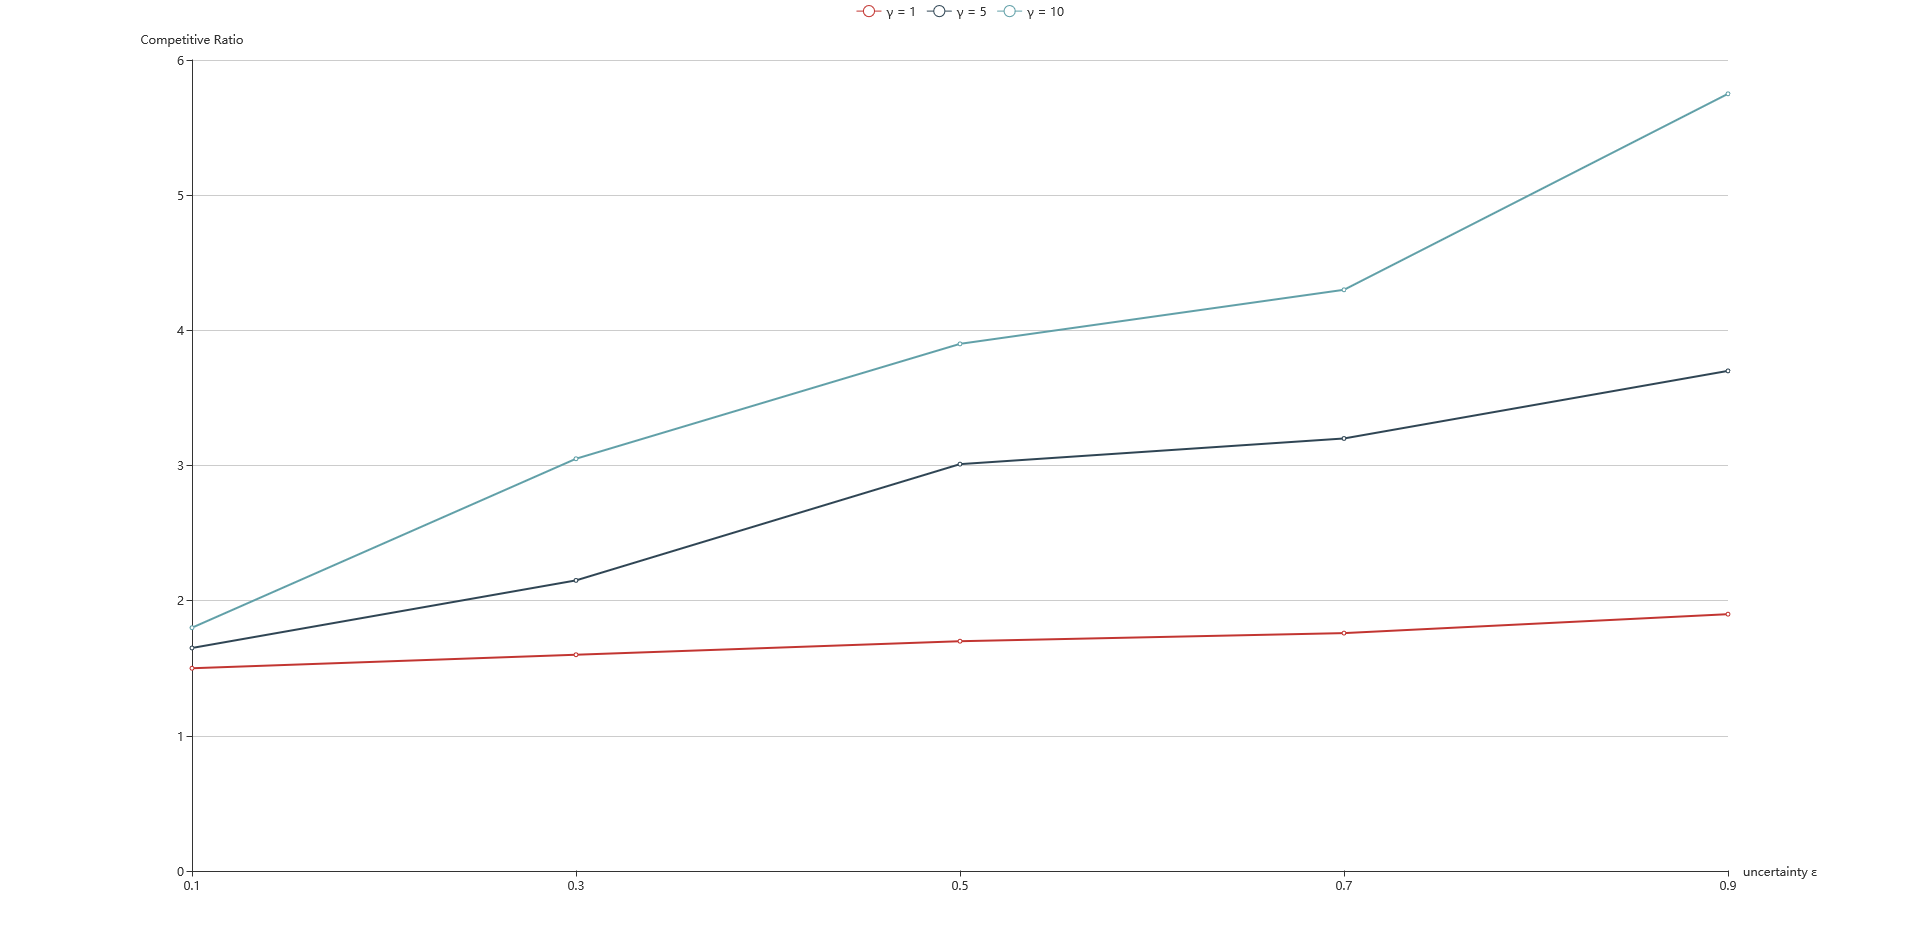
\includegraphics[height=2.4cm,width=3.8cm]{12.png}
    \caption*{(d) Competitive ratio with the uncertainty level}
    \label{fig:Competitive ratio with the uncertainty level}
    \end{minipage}
\end{figure}

In the second stage, we first fix $\epsilon =0.1$ , $m= 100$ and $\gamma =5$ to explore the relationship between time horizon $T$ and the overall cost of Online Problem and Offline Problem. As we can see, as T increases, the overall cost also increases but the online cost has never deviated from the offline optimal much. It is similar when we change the number of VNFs, which means our algorithm provides with an acceptable result.

In addition, we evaluate the effects of uncertainty $\epsilon$ and penalty ratio $\gamma$ on the competitive ratio with fixed T(100) and number of VNFs(50). As we can see, the competitive ratio rises when $\epsilon$ or $\gamma$ increases. However, in reality, $\epsilon$ and $\gamma$ cannot be that high. Therefore, our algorithm works well even with large penalty ratios and high uncertainty level.

\section{Conclusion}
In this project, we studied the problem of NFV chain scheduling on multi-core servers and proposed a two-stage optimization framework. We mainly focus on the first stage of the problem. We prove the hardness of the first stage and propose an approximation algorithm for it. Then we design an online algorithm for the second stage. Our evaluation results show that our algorithm for the first stage has excellent time performance while maintaining near-optimal property (96.9$\%$ optimal rate) and our algorithm for the second stage leads to significantly low competitive ratios.




\section{Acknowledgements}
\\\indent We are grateful to professor Li Jiang who gives us the chance to work on this project by applying what we have learned in the Algorithm Design curriculum, such as the complexity analysis and the approximation algorithm design. We are also grateful to him for his inspiration on the design of the approximation algorithms. 
\\\indent We are also thankful the teaching assistants who help professor Li Jiang to organize the presentations of the project. 








% Bibliography
\begin{thebibliography}{99}
\bibitem{c1}
M. C. Luizelli, D. Raz, and Y. S. ’Ar. Optimizing NFV chain deployment through minimizing the cost of virtual switching. In INFOCOM, pages
1–9, 2018.
\bibitem{c2}
M. C. Luizelli, D. Raz, Y. Sa’ar, and J. Yallouz. The actual cost of software switching for NFV chaining. In IM, pages 335–343, 2017.
\bibitem{c3}
M. Shi, X. Lin, S. Fahmy, and D.-H. Shin. Competitive online convex optimization with switching costs and ramp constraints. In INFOCOM, pages 1–9, 2018.
\bibitem{c4}
M. Ghaznavi, A. Khan, N. Shahriar, K. Alsubhi, R. Ahmed, and
R. Boutaba. Elastic virtual network function placement. In CloudNet, pages 255–260, 2015.
\bibitem{c5}
W. Ma, O. Sandoval, J. Beltran, D. Pan, and N. Pissinou. Traffic aware placement of interdependent NFV middleboxes. In INFOCOM, pages 1–9, 2017.
\bibitem{c6}
Y. Sang, B. Ji, G. R. Gupta, X. Du, and L. Ye. Provably efficient algorithms for joint placement and allocation of virtual network functions. In INFOCOM, pages 1–9, 2017.
\bibitem{c7}
S. G. Kulkarni, W. Zhang, J. Hwang, S. Rajagopalan, K. K. Ramakrishnan, T. Wood, M. Arumaithurai, and X. Fu. Nfvnice: Dynamic backpressure and scheduling for NFV service chains. In SIGCOMM, pages 71–84, 2017.
\bibitem{c8}
X. Wang, C. Wu, F. Le, and F. C. Lau. Online learning-assisted vnf service chain scaling with network uncertainties. In CLOUD, pages 205–213, 2017.
\bibitem{c9}
A. Ben-Tal, L. El Ghaoui, and A. Nemirovski. Robust Optimization.
Princeton University Press, 2009.
\end{thebibliography}


\end{document}
